\section{Type de matériel recommandé}

\paragraph{} L'infrastructure supportant notre système de machines virtuelles
est un système complexe, composé de nombreuses briques dont le rôle est défini.
Il faut donc soigneusement définir le type de matériel, afin que chaque élément
corresponde aux tâches qu'il aura à remplir.

\paragraph{} Si on regarde le système dans son ensemble, on compte cinq grands
ensembles de matériel à étudier. Les serveurs composeront le coeur du
système et auront pour fonction principale d'exécuter les machines virtuelles.
On dissociera les serveurs d'exécutions de ceux chargés de gérer le stockage des
données : ces derniers ont des besoins spécifiques qui doivent être couverts.
Les postes clients permettent aux utilisateurs d'accéder aux machines virtuelles
exécutées à distance, il faut donc également prévoir l'infrastructure réseau qui
sera en mesure de gérer ce trafic. Enfin, on évaluera l'infrastructure
nécessaire au support du système, notamment la fourniture d'électricité, le
stockage du matériel et des serveurs ou encore la sécurité.

\begin{figure}[h]
  \caption{\label{archi_materiel} Synoptique de l'infrastructure}
  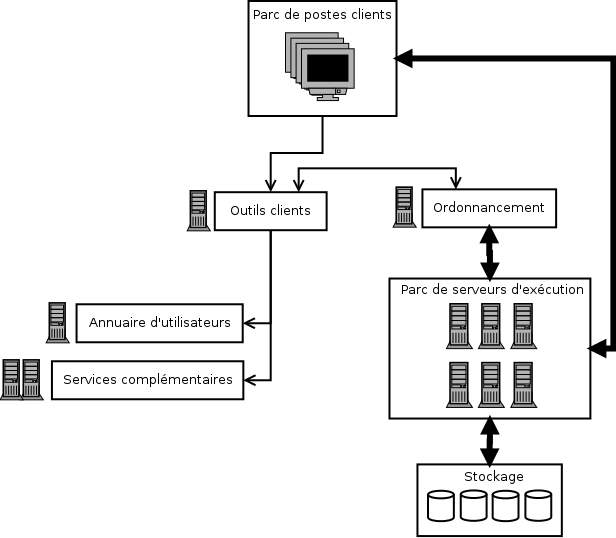
\includegraphics[scale=0.6]{archi_materiel.png}
\end{figure}

\paragraph{} La figure \ref{archi_materiel} présente une vue d'ensemble de
l'interaction entre les serveurs composant le coeur du système, les postes
clients et le stockage. Ces différents éléments seront présentées dans les
sections suivantes.

\subsection{Serveurs}

\paragraph{} On discutera, dans cette section, du coeur du système, c'est à dire
du parc de serveurs supportant l'ordonnancement et l'exécution des machines
virtuelles, la gestion de l'annuaire des utilisateurs et les outils clients
d'administration et de gestion des machines.

\subsubsection{Vue d'ensemble}

\paragraph{} Le serveur \emph{Outils clients} sera le premier sollicité : il sera
utilisé pour fournir aux utilisateurs les outils d'administration et de gestion
des machines virtuelles. Par exemple, lorsqu'un utilisateur souhaite accéder à
une machine depuis un poste client, il devrai s'authentifier sur ce serveur, qui
en retour, lui fournira la liste des machines virtuelles avec lesquelles il peut
interagir et les actions qu'il peut effectuer. Ce serveur est un élément
critique du système.

\paragraph{} Le serveur \emph{Ordonnancement} reçoit les demandes des
utilisateurs par le biais du serveur \emph{Outils clients}, il a pour rôle de
gérer l'allocation des ressources et l'exécution des machines virtuelles sur les
noeuds d'exécution. Même si il ne communique pas directement avec les postes
clients, c'est un noeud critique du système, car il supervise le système et
assure son bon fonctionnement.

\paragraph{} Ces deux serveurs sont critiques : leur bon fonctionnement est
nécessaire pour que le système soit opérationnel. Nous devons donc sélectionner
du matériel offrant un très haut niveau de fiabilité et des garanties de
sécurité de fonctionnement.

\paragraph{} Les serveurs de services (\emph{Annuaire d'utilisateurs} et
\emph{Services complémentaires}) doivent également offrir des garanties de
fonctionnement. Celles-ci sont déterminées en fonction de la criticité du
système. On peut considérer que le serveur d'annuaire est également critique.

\paragraph{} La figure \ref{archi_materiel} montre que les serveurs \emph{Outils
client}, \emph{Ordonnancement}, \emph{Annuaire d'utilisateurs} et \emph{Services
complémentaires} sont des unités distinctes. En réalité, l'organisation de ces
serveurs dépend de la configuration de l'infrastructure et du volume de la
sollicitation des différents services. Bien souvent, l'annuaire sera
effectivement sur un serveur autonome. Cependant, les serveurs
\emph{Ordonnancement} et \emph{Outils clients} ont les mêmes exigences de
matériel, et peuvent être réunis dans un seul serveur.

\paragraph{} Les noeuds d'exécutions sont sollicités pour fournir des ressources
(mémoire vive et temps d'exécution du processeur). On peut voir le parc de ces
serveurs comme un ensemble homogène qui répond à des requêtes de l'ordonnanceur
et des clients utilisant leur machine virtuelle.

\paragraph{} Le dysfonctionnement d'un des noeuds provoquera une dégradation du
service, mais n'empêche pas son fonctionnement dans l'ensemble. Un noeud
défaillant ne pénalisera que les clients pour lesquels il exécute des machines
virtuelles.

\paragraph{} En revanche, ces serveurs doivent offrir d'excellentes
performances, et doivent être équipés en conséquence. On privilégiera une
architecture très rapide, à base de processeurs optimisés pour la virtualisation
tels que les processeurs \emph{Intel Xeon} disposant de l'ensemble de
technologies regroupées sous le terme commercial \emph{Intel VT-x}. Ces serveurs
seront équipée de mémoire RAM rapide et de disques SSD dont la capacité de
stockage sera limitée : un hyperviseur bare-metal tiendra largement sur 16 Go.

\subsubsection{Serveurs haute disponibilité}

\paragraph{} Ce profil de matériel doit être utilisé pour les serveurs critiques
(\emph{Ordonnancement} et \emph{Outils clients}). Ces serveurs disposent d'une
architecture sécurisé par redondance : si l'un des éléments est défaillant, le
second reste opérationnel et peut fournir un service dégradé.

\paragraph{} Un tel serveur doit disposer de ces fonctionnalités : 

\begin{description}
  \item[Carte mère et processeurs] Une carte mère haute disponibilité doit
  disposer de deux sockets pour processeurs, supporter la téchnologie ECC pour
  la mémoire vive et la réplication des données en RAID 1 (présentés
  ci-dessous).
  \item[Mémoire vive ECC] La mémoire vive (RAM) ECC, pour \emph{Error
  Correcting-Code} permet de détecter et prévenir activement la corruption des
  données dans la mémoire vive. Ce type de mémoire est très courant sur les
  serveurs.
  \item[Réplication des données] L'utilisation d'une technologie RAID supportée
  par le matériel duplique temps réel toutes les opérations d'écritures sur le
  disque sur un second, afin de garantir l'intégrité des données, sans impact
  sur les performances.
  \item[Stockage] Un tel serveur doit disposer d'un espace de stockage limité et
  sécurisé : 2 disques durs de 500 Go montés en RAID sont suffisants.
  \item[Réseau] Deux interfaces réseau doivent être déployées pour garantir la
  disponibilité du système. Ces interfaces doivent supporter un volume de
  trafic important, et doivent supporter un volume de 1GB/s symétrique.
  \item[Performances] Afin de supporter les pics d'activité, ce serveur sera
  équipé 2 barrettes 4 Go de mémoire vive ECC installées en parallèle.
\end{description}

\subsubsection{Serveurs d'exécution}

\paragraph{} Ce profil de matériel est conçu pour privilégier les performances
de calcul brutes. Il est possible d'utiliser en parallèle plusieurs serveurs
dont les performances varient. Généralement, on préférera manipuler un nombre de
serveurs limités afin d'économiser des ressources comme la place et
l'électricité.

\paragraph{} Ces serveurs doivent être équipés de ce type de matériel :

\begin{description}
  \item[Processeurs] 2 à 4 processeurs optimisés pour la virtualisation, tels
  que les processeurs \emph{Intel i7} ou \emph{Intel Xeon}, offrant au moins 4
  coeurs et un cache mémoire important.
  \item[Mémoire vive] Ces serveurs doivent être en mesure d'accueillir en
  mémoire vive l'équivalent de plusieurs postes clients (système
  d'exploitation et logiciels utilisateurs), et donc doivent disposer de
  beaucoup de mémoire. On propose d'équiper ces serveurs de 4 x 16 Go.
  \item[Stockage] les besoins de stockages étant restreints, on propose
  d'équiper ces serveurs d'un disque SSD de 16Go.
  \item[Interfaces réseau] Ces serveurs doivent supporter le trafic généré par
  le déport d'affichage d'une part, et pouvoir accéder aux serveurs de stockage
  avec un impact limité sur les performances. Il est donc nécessaire d'équiper
  ces serveurs d'interfaces réseau de grande capacité, soit 10GB/s symétrique.
\end{description}

\subsection{Stockage}

\paragraph{} Les serveurs de stockage sont optimisés pour supporter de gros
volumes de données et des hautes performances en entrée/sortie. Ils doivent en
outre supporter des technologies de réplication de données pour garantir
l'intégrité et la sécurité des données. Ces serveurs n'ont, en revanche, pas
besoins de grosses capacités de calcul.

\paragraph{} TODO

\subsection{Réseau}

\paragraph{Support}

\subsection{Postes clients}

\subsection{Analyse de l'existant}

voir avec les admins
